% couette-flow-2D.tex

\newpage
\section{Couette Flow}
\label{couette-flow-2D}\index{boundary conditions!MovingWallBC!example of use}
%
This case is contributed by Jason Qin and computes the Couette flow between two parallel plates,
one is a moving wall with a translational velocity while the other stationary wall.
The flow is driven by the virtue of viscous drag force acting on the fluid and the applied
pressure gradient parallel to the plates.
This test case exercises the \emph{moving-wall} boundary condition.

\medskip
The boundary conditions are shown in Figure~\ref{couette-layout-fig}, 
with the NORTH and SOUTH faces set as the moving-wall and adiabatic boundary conditions, respectively.
The velocity of the NORTH face is set as 100\,m/s.
The function \verb!connect_blocks_2D! is used to connect the WEST and EAST faces, 
which can be regarded as periodic boundary conditions.

\begin{figure}[htbp]
\begin{center}
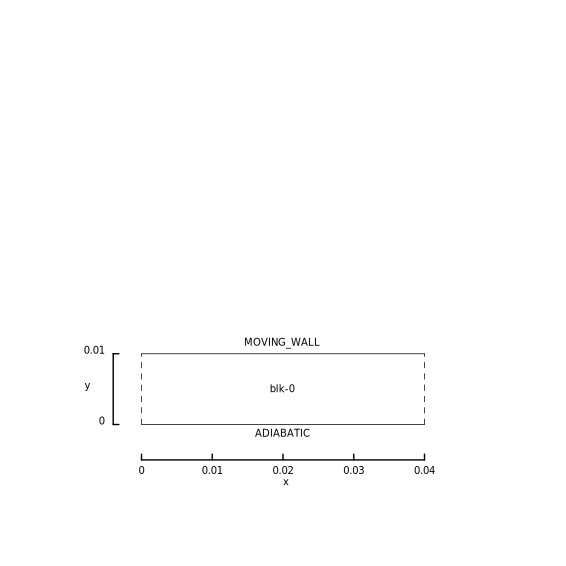
\includegraphics[width=0.7\textwidth]{../2D/couette-flow/couette.pdf}
\end{center}
\caption{Flow domain for viscous flow between two parallel plates.}
   \label{couette-layout-fig}
\end{figure}

\medskip
The mesh of $20 \times 10$ for this simple domain is plotted in Figure~\ref{fig:couette-mesh} 
and the velocity coutour is shown in Figure~\ref{fig:couette-velocity}.
The maximum velocity at is approximately 95\,m/s, 
slightly less than the translational velocity of moving wall, 
as expected for a cell-centre value.

\begin{figure}[htbp]
 \centering
 \subfloat[Mesh.]{\includegraphics[width=0.45\textwidth]
    {../2D/couette-flow/c_2D_mesh.png}\label{fig:couette-mesh}}
 \rule{2mm}{0mm}
 \subfloat[Velocity magnitude.]{\includegraphics[width=0.45\textwidth]
    {../2D/couette-flow/c_2D_velocity_counter.png}\label{fig:couette-velocity}}
 \caption{Uniform mesh and resulting velocity field for the two-dimensional Couette flow example.}
 \label{couette-mesh-and-velocity-fig}
\end{figure}

Since the initial velocity profile along the height is set as linear, 
the solution achieves steady state condition quickly.
The final velocity profile is the same as the initial profile, 
as shown in Figure~\ref{couette-velocity-profile-fig}.

\begin{figure}[htbp]
\begin{center}
\includegraphics[width=0.8\textwidth,viewport=38 49 422 302,clip=true]{../2D/couette-flow/velocity.pdf}
\end{center}
\caption{Velocity profile across the channel.}
   \label{couette-velocity-profile-fig}
\end{figure}

\bigskip
\subsection{Input script (.py)}
\topbar
\lstinputlisting[language={}]{../2D/couette-flow/couette.py}
\bottombar

\subsection{Shell scripts}
\label{couette-flow-2D-sh-files}
\topbar
\lstinputlisting[language={}]{../2D/couette-flow/couette.sh}
\bottombar

\subsection{Notes}
\begin{itemize}
\item None
\end{itemize}


